\chapter{SSA destruction for machine code \Author{F. Rastello}}
\inputpath[figs]{part4}{alternative_ssa_destruction_algorithm}
\inputprogress


\label{chapter:alternative_ssa_destruction_algorithm}
\index{interference}
\index{SSA destruction}


\section{Introduction}
Chapter~\ref{chapter:classical_construction_algorithm} provides a basic algorithm for destructing SSA that suffers from several limitations and drawbacks: 
first, it works under implicit assumptions that are not necessarily fulfilled at machine level; 
second, it must rely on subsequent phases to remove the numerous copy operations it inserts; 
finally, it increases subsequently the size of the intermediate representation, thus making it not suitable for just-in-time compilation.

\paragraph{Correctness}
SSA at machine level\index{SSA, machine level} complicates the process of destruction\index{SSA, destruction} that can potentially lead to bugs if not performed carefully. 
The algorithm described in Section~\ref{sec:classical_construction_algorithm:destruction} involves the splitting of every critical edge\index{critical edge}. 
Unfortunately, because of specific architectural constraints, region boundaries, or exception handling code, edge splitting\index{edge splitting} is not always possible. 
As we will see further, this obstacle could easily be overcome by appending copy operations at the very beginning and very end of basic blocks. 
Unfortunately, appending a copy operation at the very end of a basic block might neither be possible (it has to be before the jump operation). 
Also, care must be taken with duplicated edges\index{duplicated edges}, i.e., when the same basic block appears twice in the list of predecessors. 
This can occur after control-flow graph structural optimizations such as dead code elimination\index{dead code elimination} or empty block elimination\index{empty block elimination}... 

SSA imposes a strict discipline on variable naming: 
every ``name'' must be associated to only one definition which is obviously most of the time not compatible with the instruction set of the targeted architecture. 
As an example, a two-address mode instruction\index{two-address mode}, such as auto-increment ($x=x+1$) would enforce its definition to use the same resource as one of its arguments (defined elsewhere), thus imposing two different definitions for the same temporary variable. 
This is why some compiler designers prefer using, for SSA construction, the notion of versioning\index{variable version} in place of renaming\index{renaming, of variables}. 
Implicitly, two versions of the same original variable should not interfere, while two names can.
Such a flavor corresponds to the C-SSA form\index{conventional SSA, C-SSA}  described in Chapter~\ref{chapter:properties_and_flavours}.
The former simplifies the SSA destruction phase, while the latter simplifies and allows more transformations to be performed under SSA (updating C-SSA is very difficult)\index{SSA, updating}. 
Apart from dedicated registers\index{dedicated registers} for which optimizations are usually very careful in managing there live range, register constraints related to calling conventions\index{calling conventions} or instruction set architecture\index{instruction set architecture!ISA} might be handled by the register allocation phase. 
However, as we will see, enforcement of register constraints impacts the register pressure as well as the number of copy operations. 
For those reasons we may want those constraints to be expressed earlier (such as for the pre-pass scheduler), in which case the SSA destruction phase might have to cope with them.

\paragraph{Code quality}
The natural way of lowering \phifuns\index{\phifun, lowering} and expressing register constraints is through the insertion of copies\index{copie, insertion} (when edge-splitting is not mandatory as discussed above). 
If done carelessly, the resulting code will contain many temporary-to-temporary copy operations. 
In theory, reducing the number of these copies is the role of the coalescing during the register allocation phase. 
A few memory and time-consuming existing coalescing heuristics mentioned in Chapter~\ref{chapter:register_allocation} are quite effective in practice. 
The difficulty comes both from the size of the interference graph (the information of colorability is spread out) and the presence of many overlapping live ranges that carry the same value (so non-interfering). 
Coalescing can also, with less effort, be performed prior to the register allocation phase. 
As opposed to a (so-called conservative\index{coalescing, conservative}) coalescing during register allocation, this aggressive coalescing\index{coalescing, aggressive} would not cope with the interference graph colorability. 
As we will see, strict SSA form is really helpful for both computing and representing equivalent variables. 
This makes the SSA destruction phase the right candidate for eliminating (or not inserting) those copies.

\paragraph{Speed and Memory Footprint}
The cleanest and simplest way to perform SSA destruction with good code quality is to first insert copy instructions to make the SSA form conventional\index{conventional SSA!C-SSA}, then take advantage of the SSA form to run efficiently aggressive coalescing (without breaking the conventional property), before eventually renaming \phiwebs\index{\phiweb} and getting rid of \phifuns. 
Unfortunately this approach will lead, in a transitional stage, to an intermediate representation with a substantial number of variables: 
the size of the liveness sets and interference graph classically used to perform coalescing become prohibitively large for dynamic compilation. 
To overcome this difficulty one can compute liveness and interference on demand which, as we already mentioned, is made simpler by the use of SSA form (see Chapter~\ref{chapter:ssa_tells_nothing_of_liveness}). 
Remains the process of copy insertion itself that might still take a substantial amount of time. 
To fulfill memory and time constraints imposed by just-in-time compilation\index{just-in-time compiler!JIT} , one idea is to \emph{virtually} insert those copies, and only \emph{effectively} insert the non-coalesced ones.

This chapter addresses those three issues: 
handling of machine level constraints, code quality (elimination of copies), and algorithm efficiency (speed and memory footprint). 
The layout falls into three corresponding sections.

\section{Correctness}

\paragraph{Isolating \phinode using copies}
In most cases, edge splitting can be avoided by treating \phiuses and \phidef symmetrically: 
instead of just inserting copies on the incoming control-flow edges of the \emph{\phinode} (one for each use operand), a copy is also inserted on the outgoing edge (one for its defining operand). 
This has the effect of isolating the value associated to the \phinode thus avoiding (as discussed further) SSA destruction issues such as the well-known lost-copy problem\index{lost-copy problem}. 
The process of \phinode isolation\index{isolation, of \phinode} is illustrated by Figure~\ref{fig:phi_isolation}. 
The corresponding pseudo-code is given in Algorithm~\ref{alg:alternative_ssa_destruction:sreedhar}. 
If, because of different \phifuns, several copies are introduced at the same place, they should be viewed as parallel copies\index{parallel copies}. 
For that reason, an empty parallel copy is initially inserted both at the beginning (i.e., right after \phifuns, if any) and at the end of each basic block (i.e., just before the branching operation, if any). 
Note that, as far as correctness is concerned, those copies can be sequentialized in any order, as they concern different variables (this is a consequence of \phinode isolation -- see below).

\begin{figure}[h]
  \hfill
\subfloat[Initial code]{
  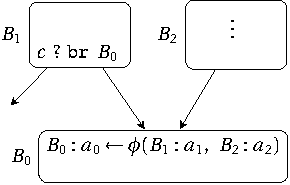
\includegraphics[scale=0.7]{phi_isolation_a.pdf}
}\hfill
\subfloat[After isolating the \phifun]{
  \hspace{2em}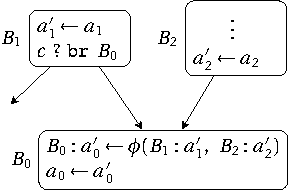
\includegraphics[scale=0.7]{phi_isolation_b.pdf}
}
\hfill\strut
\caption{Isolation of a \phinode\label{fig:phi_isolation}\index{isolation, of \phinode}}
\end{figure}


When incoming edges are not split, inserting a copy not only for each argument of the \phifun, but also for its result is important: 
without the copy $a'_0\gets a_0$, the \phifun defines directly~$a_0$ whose live range can be long enough to intersect the live range of some $a'_i$, $i>0$. 
Prior SSA destruction algorithms that did not perform the copy  $a'_0\gets a_0$ identified two problems.
(1)~In the ``lost-copy problem''\index{lost-copy problem},  $a_0$ is used in a successor of $B_i \neq B_0$, and the edge from~$B_i$ to~$B_0$ is \emph{critical}.
(2)~In the ``swap problem''\index{swap problem}, $a_0$ is used in $B_0$ as a \phifun argument. 
In this latter case, if parallel copies\index{parallel copies} are used, $a_0$ is dead before~$a'_i$ is defined.
But, if copies are sequentialized blindly, the live range of~$a_0$ can go beyond the definition point of~$a'_i$ and lead to an incorrect code after renaming $a_0$ and $a'_i$ with the same name. 
\phinode isolation allows to solve most of the issues that can be faced at machine level. 
However, there remains subtleties listed below.


\paragraph{Limitations}
There is a tricky case, when the basic block contains variables \emph{defined after} the point of copy insertion. 
This is for example the case for the PowerPC \texttt{bclr} branch instructions\index{branch instruction problem} with a behavior similar to hardware loop\index{hardware loop}. 
In addition to the condition, a counter $u$ is decremented by the instruction itself. 
If $u$ is used in a \phifun in a direct successor block, no copy insertion can split its live range. 
It must then be given the same name as the variable defined by the \phifun. 
If both variables interfere, this is just impossible! 
For example, suppose that for the code of Figure~\ref{fig:alternative_ssa_destruction:ex_jump_impossible_a}, the instruction selection chooses a branch with decrement (denoted \texttt{br\_dec}) for Block~$B_1$ (Figure~\ref{fig:alternative_ssa_destruction:ex_jump_impossible_b}). 
Then, the \phifun of Block~$B_2$, which uses $u$, cannot be translated out of SSA by standard copy insertion because $u$ interferes with $t_1$ and its live range cannot be split. 
To destruct SSA, one could add $t_1\gets u-1$ in Block~$B_1$ to anticipate the branch. 
Or one could split the critical edge between $B_1$ and~$B_2$ as in Figure~\ref{fig:alternative_ssa_destruction:ex_jump_impossible_c}. 
In other words, simple copy insertions is not enough in this case.
We see several alternatives to solve the problem:
(1)~the SSA optimization could be designed with more care;
(2)~the counter variable must not be promoted to SSA;
(3)~some instructions must be changed;
(4)~the control-flow edge must be split somehow. 

\begin{figure}[h]
\subfloat[Initial SSA code]{
    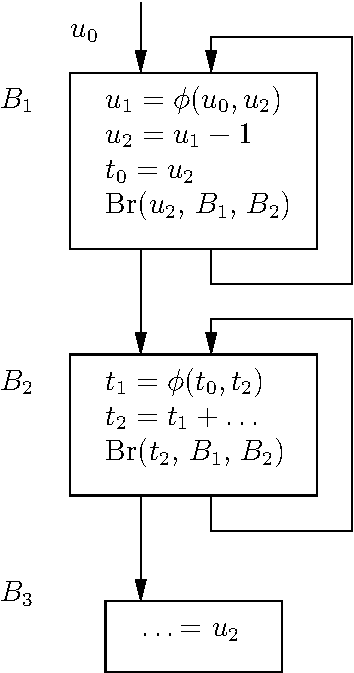
\includegraphics[scale=0.7]{cexple-impossible-1.pdf}\label{fig:alternative_ssa_destruction:ex_jump_impossible_a}
}
\hfill
\subfloat[Branch with decrement]{
    \hspace{2em}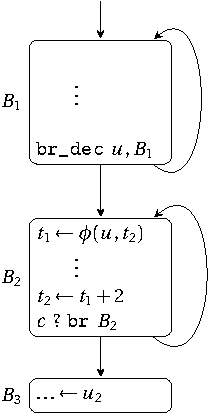
\includegraphics[scale=0.7]{cexple-impossible-2.pdf}\hspace{2em}\label{fig:alternative_ssa_destruction:ex_jump_impossible_b}
}
\hfill
\subfloat[C-SSA with additional edge splitting]{
    \hspace{1em}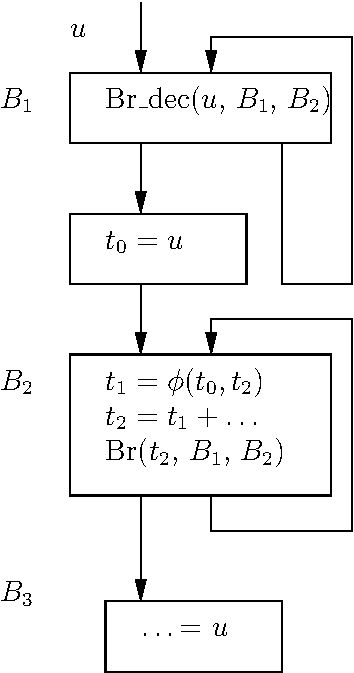
\includegraphics[scale=0.7]{cexple-impossible-3.pdf}\hspace{1em}\label{fig:alternative_ssa_destruction:ex_jump_impossible_c}
}
\caption{Copy insertion may not be sufficient\index{branch instruction problem}. $\texttt{br\_dec}\ u,B_1$ decrements $u$, then branches to $B_1$ if $u\neq 0$.\label{fig:alternative_ssa_destruction:ex_jump_impossible}}
\end{figure}

There is another tricky case when a basic block has twice the same predecessor block\index{duplicated edge problem}. 
This can result from consecutively applying copy-folding and control-flow graph structural optimizations such as dead code elimination\index{dead code elimination} or empty block elimination\index{empty block elimination}. 
This is the case for the example of Figure~\ref{fig:alternative_ssa_destruction:doublepreds} where copy-folding\index{copy-folding} would remove the copy $a_2\gets b$ in Block~$B_2$. 
If $B_2$ is eliminated, there is no way to implement the control dependence of the value to be assigned to $a_3$ other than through predicated code (see chapters~\ref{chapter:psi_ssa} and~\ref{chapter:vsdg}) or through the reinsertion of a basic block between $B_1$ and $B_0$ by the split of one of the edges.

\begin{figure}[h]
\subfloat[Initial C-SSA code]{
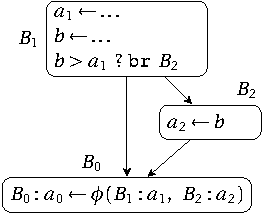
\includegraphics[scale=0.7]{doublepreds_a.pdf}
}\hfill
\subfloat[T-SSA code]{
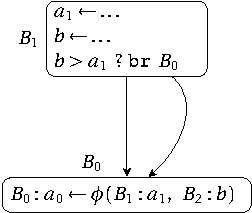
\includegraphics[scale=0.7]{doublepreds_b.pdf}
}\hfill
\subfloat[After $\phi$-isolation]{
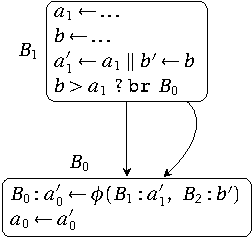
\includegraphics[scale=0.7]{doublepreds_c.pdf}
}\caption{\label{fig:alternative_ssa_destruction:doublepreds} Copy-folding followed by empty block elimination can lead to SSA code for which destruction is not possible through simple copy insertion\index{duplicated edge problem}}
\end{figure}


The last difficulty SSA destruction faces when performed at machine level is related to register constraints such as instruction set architecture (ISA)\index{instruction set architecture|ISA} or application binary interface (ABI)\index{application binary interface|ABI} constraints. 
For the sake of the discussion we differentiate two kinds of resource constraints that we will refer as \emph{operand pinning}\index{pinning} and \emph{live range pinning}\index{live range pinning}. 
The live range pinning of a variable $v$ to resource $R$ will be represented $R_v$, just as if $v$ were a version of temporary $R$. 
An operand pinning to a resource $R$ will be represented using the exponent $\pining{R}$ on the corresponding operand. 
Live range pinning expresses the fact that the \emph{entire} live range of a variable must reside in a given resource (usually a dedicated register). 
An example of live range pinning are versions of the stack-pointer temporary that must be assigned back to register \SP\index{stack pointer}. 
On the other hand, the pinning of an operation's operand to a given resource does not impose anything on the live range of the corresponding variable. 
The scope of the constraint is restricted to the operation. 
Examples of operand pinning are operand constraints such as \emph{two-address mode}\index{two-address mode} where two operands of one instruction must use the same resource; 
or where an operand must use a given register. 
This last case encapsulates ABI constraints.
\begin{figure}[h]
\subfloat[Operand pinning of an auto-increment]{
  \begin{minipage}{0.45\textwidth}
~\\
    \centerline{$p_2\pining{T}\gets p_1\pining{T}+1$}
~\\
  \end{minipage}
}
\hfill
\subfloat[Corresponding live range pinning]{
  \hspace{3em}\begin{minipage}{0.35\textwidth}
    $T_{p_1}\gets p_1$\\
    $T_{p_2}\gets T_{p_1}+1$\\
    $p_2\gets T_{p_2}$
  \end{minipage}
}
\\
\subfloat[Operand pinning of a function call]{
  \begin{minipage}{0.4\textwidth}
~\\
    \centerline{$a\pining{R0}\gets f(b\pining{R0}, c\pining{R1})$}
~\\  \end{minipage}
}
\hfill
\subfloat[Corresponding live range pinning]{
  \hspace{3em}\begin{minipage}{0.35\textwidth}
    ${R0}_{b'}=b\ \parallel\ {R1}_{c'}=c$\\
    ${R0}_{a'}=f({R0}_{b'},{R1}_{c'})$\\
    $a={R0}_{a'}$
  \end{minipage}
}
\caption{\label{fig:alternative_ssa_destruction:pining}Operand pinning and corresponding live range pinning}
\end{figure}

Note that looser constraints where the live range or the operand can reside in more than one resource are not handled here. 
We assume that the handling of that last constraint is the responsibility of the register allocation. 
We first simplify the problem by transforming any operand pinning to a live range pinning as sketched in Figure~\ref{fig:alternative_ssa_destruction:pining}: 
parallel copies with new variables pinned to the corresponding resource are inserted just before (for \useop pinning) and just after (for \defop pinning) the operation.




\paragraph{Detection of strong interferences}
\label{par:alternative_ssa_destruction:strong}
The scheme we propose in this section to perform SSA destruction that deals with machine level constraints does not address compilation cost (in terms of speed and memory footprint). 
It is designed to be simple. 
It first inserts parallel copies\index{parallel copies} to isolate \phifuns and operand pinning. 
Then it checks for interferences that would persist. 
We will denote such interferences as \emph{strong}\index{interference, strong}, as they cannot be tackled through the simple insertion of temporary-to-temporary copies in the code. 
We consider that fixing strong interferences should be done on a case-by-case basis and restrict the discussion here on their detection.

As far as correctness is concerned, Algorithm~\ref{alg:alternative_ssa_destruction:sreedhar} splits the data flow between variables and \phinodes through the insertion of copies. 
For a given \phifun $a_0\gets \phi(a_1,\dots,a_n)$, this transformation is correct as long as the copies can be inserted close enough to the \phifun. 
It might not be the case if the insertion point (for a \useop) of copy $a'_i\gets a_i$ is not dominated by the definition point of $a_i$ (such as for argument $u$ of the \phifun $t_1\gets \phi(u,t_2)$ for the code of Figure~\ref{fig:alternative_ssa_destruction:ex_jump_impossible_b}); 
symmetrically, it will not be correct if the insertion point (for the \defop) of copy $a_0\gets a'_0$ does not dominate all the uses of $a_0$. 
Precisely this leads to inserting in Algorithm~\ref{alg:alternative_ssa_destruction:sreedhar} the following tests:
\begin{itemize}
\item line~\ref{line:sreedhar:1}: ``{\bf if} the definition of $a_i$ does not dominate $\textit{PC}_i$ {\bf then} continue;''
\item line~\ref{line:sreedhar:2}: ``{\bf if} one use of $a_0$ is not dominated by $\textit{PC}_0$ {\bf then} continue;''
\end{itemize}
For the discussion, we will denote as \emph{split operands}\index{\phifun operands, split} the newly created local variables to differentiate them to the ones concerned by the two previous cases (designed as \emph{non-split operands}\index{\phifun operands, non-split}).
We suppose a similar process have been performed for operand pinning to express them in terms of live range pinning with very short (when possible) live ranges around the concerned operations. 

At this point, the code is still under SSA and the goal of the next step is to check that it is conventional: 
this will obviously be the case only if all the variables of a \phiweb\index{\phiweb} can be coalesced together. 
But not only: 
the set of all variables pinned to a common resource must also be interference free. 
We say that $x$ and $y$ are \emph{pin-$\phi$-related} to one another if they are $\phi$-related or if they are pinned to a common resource. 
The transitive closure of this relation defines an equivalence relation that partitions the variables defined locally in the procedure into equivalence classes, the pin-$\phi$-webs\index{pin-\phiweb}. 
Intuitively, the pin-$\phi$-equivalence class of a resource represents a set of resources ``connected'' via \phifuns and resource pinning. 
The computation of \phiwebs given by Algorithm~\ref{alg:ssadestruction:find-webs} can be generalized easily to compute pin-\phiwebs. 
The resulting pseudo-code is given by Algorithm~\ref{alg:alternative_ssa_destruction_algorithm:find-webs}.

\begin{algorithm}[h]
      \ForEach{$B$: basic block of the CFG}{
        insert an empty parallel copy at the beginning of $B$\;
        insert an empty parallel copy at the end of $B$\;
      }
      \ForEach{$B_0$: basic block of the CFG}{
        \ForEach{\phifun at the entry of $B_0$ of the form $a_0=\phi(B_1:a_1,\ldots,B_n:a_n)$}{
          \ForEach{$a_i$ (argument of the \phifun corresponding to $B_i$)}{
            \Let $PC_i$ be the parallel-copy at the end of $B_i$\;
            \nl\label{line:sreedhar:1} \BlankLine
            \Let $a'_i$ be a freshly created variable\;
            add copy $a'_i \gets a_i$ to $\mathrm{PC}_i$\;
            replace $a_i$ by $a'_i$ in the \phifun;
          }
          \Begin{
              \Let $PC_0$ be the parallel-copy at the beginning of $B_0$\;
              \nl\label{line:sreedhar:2} \BlankLine
              \Let $a'_0$ be a freshly created variable\;
              add copy $a_0 \gets a'_0$ to $\mathrm{PC}_0$\;
              replace $a_0$ by $a'_0$ in the \phifun\;
           }
          \Comment{all $a'_i$ can be coalesced and the \phifun removed}
        }
      }
 \caption{\label{alg:alternative_ssa_destruction:sreedhar}Algorithm making 
 non-conventional SSA form conventional by isolating \phinodes}
\end{algorithm}

Now, one needs to check that each web is interference free. 
A web contains variables and resources. 
The notion of interferences\index{interference} between two variables is the one discussed in Section~\ref{sec:properties_and_flavors:ultimate_interference} for which we will propose an efficient implementation later in this chapter. 
A variable and a physical resource do not interfere while two distinct physical resources interfere with one another.

If any interference has been discovered, it has to be fixed on a case-by-case basis. 
Note that some interferences such as the one depicted in Figure~\ref{fig:alternative_ssa_destruction:doublepreds} can be detected and handled initially (through edge splitting if possible) during the copy insertion phase.


\begin{algorithm}[h]
%% proc find_webs
%% // find the ssa web of each variable
\For{each resource $R$}{
  $\mathrm{web}(R)\gets \{R\}$\;
}
\For{each variable $v$}{
  $\mathrm{web}(v) \leftarrow \{v\}$\;
  \If{$v$ pinned to a resource $R$}{
    union$(\mathrm{web}(R),\mathrm{web}(v))$
 }
}
\For{each instruction of the form $a_{\mathrm{dest}} = \phi(a_1,\ldots,a_n)$}{
  \For{each source operand $a_i$ in instruction}{
     union$(\mathrm{web}(a_{\mathrm{dest}}),\mathrm{web}(a_i))$
  }
}
\caption{\label{alg:alternative_ssa_destruction_algorithm:find-webs}The pin-\phiwebs discovery algorithm, based on the union-find pattern\index{\phiweb, discovery}}
\end{algorithm}

\section{Code Quality}
\label{sec:destruct:quality}
Once the code is in conventional SSA, the correctness problem is solved: 
destructing it is by definition straightforward, as it relies in renaming all variables in each \phiweb into a unique representative name and then remove all \phifuns. 
To improve the code, however, it is important to remove as many copies as possible.

\paragraph{Aggressive coalescing}
Aggressive coalescing can be treated with standard non-SSA coalescing technique.
Indeed, conventional SSA allows to coalesce the set of all variables in each \phiweb together.
Coalesced variables are not SSA variables anymore, but \phifuns can be removed.
Liveness and interferences can then be defined as for a regular code (with parallel copies). 
An interference graph\index{interference graph} (as depicted in Figure~\ref{fig:alternative_ssa_destruction:lost-graph}) can be used. 
A solid edge between two nodes (e.g., between $x_2$ and $x_3$) materialize the presence of an interference\index{interference} between the two corresponding variables, i.e., expressing the fact that they cannot be coalesced and share the same resource. 
A dashed edge between two nodes materializes an affinity\index{affinity} between the two corresponding variables, i.e., the presence of a copy (e.g., between $x_2$ and $x'_2$) that could be removed by their coalescing.

This process is illustrated by Figure~\ref{fig:alternative_ssa_destruction:ex_lost}: 
the isolation of the \phifun leads to inserting the three copies that respectively define $x'_1$, $x'_3$, and uses $x'_2$; 
the corresponding \phiweb $\{x'_1, x'_2, x'_3\}$ is coalesced into a representative variable $x$; 
according to the interference graph of Figure~\ref{fig:alternative_ssa_destruction:lost-graph}, $x_1$, $x_3$ can then be coalesced with $x$ leading to the code of Figure~\ref{fig:alternative_ssa_destruction:lost3}.

\begin{figure}[H]
\subfloat[Lost-copy problem\index{lost-copy problem}]{
  \hspace{1em}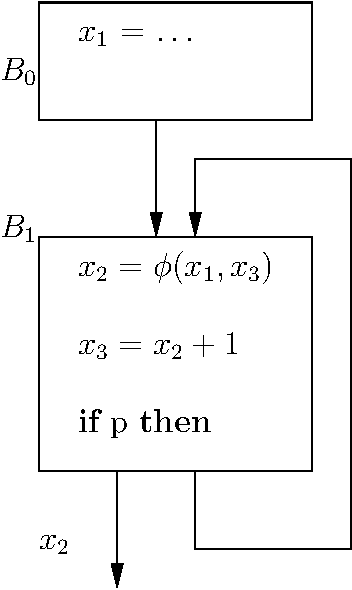
\includegraphics[scale=0.7]{lost.pdf}\hspace{1em}
}
\hfill
\begin{minipage}{0.3\textwidth}
\subfloat[C-SSA\index{isolation, of \phinode}]{
  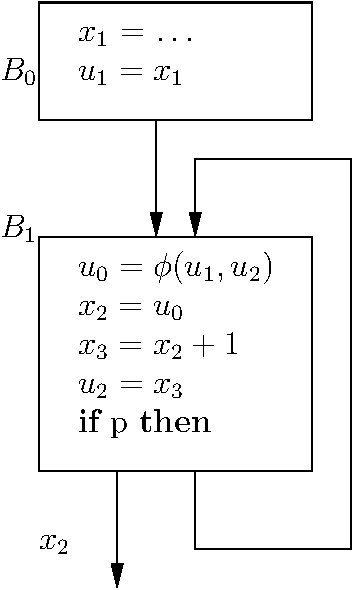
\includegraphics[scale=0.7]{lost2.pdf}
}\\
\subfloat[Interferences\label{fig:alternative_ssa_destruction:lost-graph-cssa}]{
  \hspace{1em}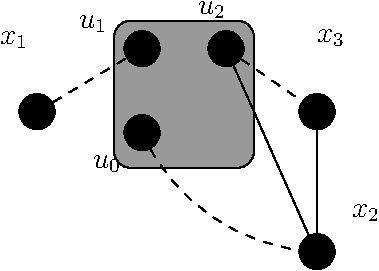
\includegraphics[scale=0.85]{lost-graph-cssa.pdf}\hspace{1em}
}
\end{minipage}
\hfill
\begin{minipage}{0.3\textwidth}
\subfloat[After coalescing\label{fig:alternative_ssa_destruction:lost3}]{
  \hspace{1em}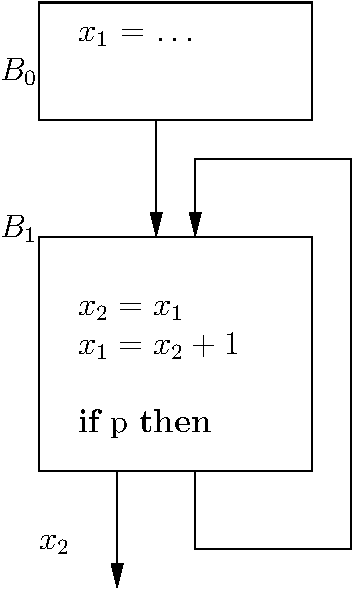
\includegraphics[scale=0.7]{lost3.pdf}\hspace{1em}
}\\\vspace{1em}~\\
\subfloat[Interferences\index{interference graph}\label{fig:alternative_ssa_destruction:lost-graph}]{
  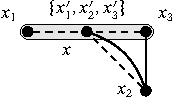
\includegraphics[scale=0.85]{lost-graph.pdf}
}
\end{minipage}
\caption{SSA destruction for the lost-copy problem.\label{fig:alternative_ssa_destruction:ex_lost}}
\end{figure}

\paragraph{Liveness under SSA}
\label{sec:alternative_ssa_destruction_algorithm:liveness}
If\index{liveness!\phifun} the goal is not to destruct SSA completely but remove as many copies as possible while maintaining the conventional property, liveness of \phifun operands should reproduce the behavior of the corresponding non-SSA code as if the variables of the \phiweb were coalesced all together. 
The semantic of the \phiop in the so-called \emph{multiplexing} mode\index{multiplexing mode, semantic of \phiop} fits the requirements. 
The corresponding interference graph on our example is depicted in Figure~\ref{fig:alternative_ssa_destruction:lost-graph-cssa}.


\begin{definition}[multiplexing mode]
  Let a \phifun $B_0:a_0=\phi(B_1:a_1,\dots,B_n:a_n)$ be in \emph{multiplexing} mode, then its liveness\index{liveness!\phifun} follows the following semantic: 
  its \defop is considered to be at the entry of $B_0$, in other words variable $a_0$ is live-in of $B_0$; 
  its \useops are at the exit\index{basic-block exit} of the corresponding predecessor basic-blocks, in other words, variable $a_i$ for $i>0$ is live-out of basic block $B_i$.
\end{definition}



\paragraph{Value-based interference}
\label{par:alternative_ssa_destruction:value}
As said earlier, after the $\phi$-isolation phase and the treatment of operand pinning constraints, the code contains many overlapping live ranges that carry the same value. 
Because of this, to be efficient coalescing must use an accurate notion of interference\index{interference, ultimate}. 
As already mentioned in Chapter~\ref{chapter:properties_and_flavours}, the ultimate notion of interference contains two dynamic (i.e., related to the execution) notions: 
the notion of liveness and the notion of value. 
Analyzing statically if a variable is live at a given execution point or if two variables carry identical values is a difficult problem. 
The scope of variable coalescing is usually not so large, and graph coloring based register allocation commonly take the following conservative test: 
\emph{two variables interfere if one is live at a definition point of the other and this definition is not a copy between the two variables\index{interference, conservative}}.

One can notice that, with this conservative interference definition, when $a$ and $b$ are coalesced, the set of interferences of the new variable may be strictly smaller than the union of interferences of $a$ and $b$. 
Thus, simply merging the two corresponding nodes in the interference graph is an over-approximation with respect to the interference definition. 
For example, in a block with two successive copies $b=a$ and $c=a$ where $a$ is defined before, and $b$ and $c$ (and possibly~$a$) are used after, it is considered that $b$ and $c$ interfere but that none of them interfere with $a$. 
However, after coalescing $a$ and $b$, $c$ should not interfere anymore with the coalesced variable. 
Hence the interference graph would have to be updated\index{interference, updating} or rebuilt.


However, in SSA, each variable has, statically, a \emph{unique} value, given by its unique definition. 
Furthermore, the ``has-the-same-value'' binary relation defined on variables is, if the SSA form fulfills the dominance property\index{dominance property} , an equivalence relation. 
The \emph{value} of an equivalence class~\footnote{Dominance property is required here, e.g., consider the following loop body $\textrm{if}(i\neq 0)$ $\{b\gets a;\}$ $c\gets\dots;$ $\dots\gets b;$ $a\gets c;$ the interference between $b$ and $c$ is actual.} 
is the variable whose definition dominates the definitions of all other variables in the class. 
Hence, using the same scheme as in SSA copy folding\index{copy-folding} , finding the value of a variable can be done by a simple topological traversal of the dominance tree: 
when reaching an assignment of a variable $b$, if the instruction is a copy $b=a$, $V(b)$ is set to $V(a)$, otherwise $V(b)$ is set to $b$. 
The interference test in now both simple and accurate (no need to rebuild/update after a coalescing): 
if $\textrm{live}(x)$ denotes the set of program points where $x$ is live,

\centerline{\emph{$a$ interfere with $b$ if $\textrm{live}(a)$ intersects
  $\textrm{live}(b)$ and $V(a)\neq V(b)$}\index{interference, value based}}

The first part reduces to $\textrm{def}(a)\in \textrm{live}(b)$ or $\textrm{def}(b)\in \textrm{live}(a)$ thanks to the dominance property. 
In the previous example, $a$, $b$, and $c$ have the same value $V(c)=V(b)=V(a)=a$, thus they do not interfere.

Note that our notion of values is limited to the live ranges of SSA variables, as we consider that each \phifun defines a new variable. 
We could propagate information through a \phifun when its arguments are equivalent (same value). 
But we would face the complexity of global value numbering\index{Global Value Numbering}  (see Chapter~\ref{chapter:pre_not_helped}). 
By comparison, our equality test in SSA comes for free.

\iffalse
\paragraph{Shared copies}
It turns out that after the $\phi$-isolation phase, and the treatment of operand pinning constraints, the code also contains \emph{shared copies}\index{shared copies}. 
A shared copy corresponds precisely to the previous example of two successive copies $b=a$ and $c=a$ i.e., the presence of two copies from the same source. 
We have seen that, thanks to our definition of value, the fact that $b$ is live at the definition of $c$ does not imply that $b$ and~$c$ interfere. 
Suppose, however, that $a$ (after some other coalescing) interferes with $b$ and $c$. 
Then, no coalescing can occur although coalescing $b$ and $c$ would save one copy, by ``sharing'' the copy of $a$. 
This sharing problem is difficult to model and optimize (the problem of placing copies is even worse), but we can optimize it a bit. 
We coalesce two variables~$b$ and~$c$ if they are both copies of the same variable~$a$ and if their live ranges intersect. 
This can be done in a second pass after all standard affinities have been treated. 
Note that if their live ranges are disjoint, such a coalescing may be incorrect as it would increase the live range of the dominating variable, possibly creating some interference not taken into account.
\fi

\section{Speed and Memory Footprint}
Implementing the technique of the previous section may be considered too costly. 
First, it inserts many instructions before realizing that most are useless.
Also, copy insertion is already by itself time-consuming. 
It introduces many new variables, too: 
The size of the variable universe has an impact on the liveness analysis and the interference graph construction. 
Finally, if a general coalescing algorithm is used, a graph representation with adjacency lists (in addition to the bit matrix) and a working graph to explicitly merge nodes when coalescing variables, would be required. 
All these constructions, updates, manipulations are time-consuming and memory-consuming. 
We may improve the whole process by: 
(a)~avoiding the use of any interference graph and liveness sets; 
(b)~avoid the quadratic complexity of interference check between two sets of variables by an optimistic approach that first coalesces all copy-related variables (even interfering ones), then traverses each set of coalesced variables and un-coalesce one by one all the interfering ones; 
(c)~emulating (``virtualizing'') the introduction of the $\phi$-related copies.

\paragraph{Interference check}
Liveness sets and interference graph are the major source of memory usage\index{interference check}. 
This motivates, in the context of JIT compilation, not to build any interference graph at all, and rely on the liveness check\index{liveness check} described in Chapter~\ref{chapter:ssa_tells_nothing_of_liveness} to test if two live ranges intersect or not. 
Let us suppose for this purpose that a ``has-the-same-value'' equivalence relation, is available thanks to a mapping $V$ of variables to symbolic values: 
\\
$$\textrm{variables }a\textrm{ and }b\textrm{ have the same value } \Leftrightarrow V(a)=V(b)$$
As explained in Paragraph~\ref{par:alternative_ssa_destruction:value} this can be done linearly (without requiring any hash map-table) on a single traversal of the program if under strict SSA form. 
We also suppose that liveness check is available, meaning that for a given variable $a$ and program point $p$, one can answer if $a$ is live at this point through the boolean value of  $a.\textit{islive}(p)$. This can directly be used, under strict SSA form, to check if two variables live ranges intersect\index{interference, intersection based}:

$$\begin{array}{rcl}
\intersect(a,b) & \Leftrightarrow & \textit{liverange}(a)\cap \textit{liverange}(b)\neq\emptyset\\
 & \Leftrightarrow & \left\lwave
\begin{array}{l}
\textit{a.def.op}=\textit{b.def.op}\\
\textit{a.def.op} \textrm{ dominates } \textit{b.def.op} \bigwedge \textit{a.islive}\left(\textit{out}(\textit{b.def.op})\right)\\
\textit{b.def.op} \textrm{ dominates } \textit{a.def.op} \bigwedge \textit{b.islive}\left(\textit{out}(\textit{a.def.op})\right)\\
\end{array}\right.
\end{array}
$$ 

Which leads to our refined notion of interference\index{interference, value based}:

$$\interfere(a,b) \Leftrightarrow \intersect(a,b) \bigwedge V(a)\neq V(b)$$ 

\paragraph{De-coalescing in linear time}
The interference check outlined in the previous paragraph allows to avoid building an interference graph of the SSA form program. 
However, coalescing has the effect of merging vertices and interference queries are actually to be done between sets of vertices. 
To overcome this complexity issue, the technique proposed here is based on a de-coalescing scheme\index{de-coalescing}. 
The idea is to first merge all copy and \phifun related variables together. 
A merged-set might contain interfering variables at this point. 
The principle is to identify some variables that interfere with some other variables within the merged-set, and remove them (along with the one they are pinned with) from the merged-set. 
As we will see, thanks to the dominance property, this can be done linearly using a single traversal of the set.

In reference to register allocation, and graph coloring, we will associate the notion of colors to merged-sets: all the variables of the same set are assigned the same color, and different sets are assigned different colors. 
The process of \emph{de-coalescing} a variable is to extract it from its set; 
it is not put in another set, just isolated. 
We will say \emph{uncolored}. 
Actually, variables pinned together have to stay together. 
We denote the (interference free) set of variables pinned to a common resource that contains variable $v$, $\atomic{v}$. 
So the process of un-coloring a variable might have the effect of un-coloring some others. 
In other words, a colored variable is to be coalesced with variables of the same color, and any uncolored variable $v$ is to be coalesced only with the variables it is pinned with, i.e.~$\atomic{v}$.


We suppose that variables have already been colored and the goal is to un-color some of them (preferably not all of them) so that each merged-set become interference free. 
We suppose that if two variables are pinned together they have been assigned the same color, and that a merged-set cannot contain variables pinned to different physical resources. 
Here we focus on a single merged-set and the goal is to make it interference free within a single traversal. 
The idea exploits the tree shape of variables live ranges under strict SSA\index{dominator!tree}. 
To this end, variables are identified by their definition point and ordered using dominance accordingly.

Algorithm~\ref{alg:alternative_ssa_destruction:domup} performs a traversal of this set along the dominance order, enforcing at each step the subset of already considered variables to be interference free. 
From now, we will abusively design as the dominators of a variable $v$, the set of variables of \emph{color identical to $v$} which definition dominates the definition of $v$. 
Variables defined at the same program point are arbitrarily ordered, so as to use the standard definition of immediate dominator (denoted $\cidom{v}$, set to $\valundef$ if not exists, updated lines~\ref{line:curidom_start}-\ref{line:curidom_end}). 
To illustrate the role of $\eanc{v}$ in Algorithm~\ref{alg:alternative_ssa_destruction:domup}, let us consider the example of Figure~\ref{fig:alternative_ssa_destruction:fig:domtree} where all variables are assumed to be originally in the same merged-set: 
$\eanc{v}$ (updated line~\ref{line:eanc}) represents the immediate intersecting dominator with the same value than $v$; 
so we have $\eanc{b}=\valundef$ and $\eanc{d}=a$. 
When line~\ref{line:curanc} is reached, $\curanc$ (if not $\valundef$) represents a dominating variable interfering with $v$ and with the same value than $\cidom{v}$: 
when $v$ is set to $c$ ($\cidom{c}=b$), as $b$ does not intersect $c$ and as $\eanc{b}=\valundef$, $\curanc=\valundef$ which allows to conclude that there is no dominating variable that interfere with $c$; 
when $v$ is set to $e$, $d$ does not intersect $e$ but as $a$ intersects and has the same value than $d$ (otherwise $a$ or $d$ would have been uncolored), we have $\eanc{d}=a$ and thus $\curanc=a$. 
This allows to detect on line~\ref{line:interference} the interference of $e$ with $a$.

\begin{algorithm}[h]
$\curidom=\valundef$\;
\ForEach{variable $v$ of the merged-set in DFS pre-order of the dominance tree}{
  \textsf{DeCoalesce}($v$, $\curidom$)\;
  $\curidom \gets v$\;
}
% \BlankLine
\BlankLine
% \BlankLine
% \BlankLine
\BlankLine
\Func{DeCoalesce($v$, $u$)}{
  %% \Comment{Finds and set the immediate dominator of $v$}
 
  \lWhile{$(u \neq \valundef) \bigwedge \left(\neg(u \dominates\ v) \vee \uncolored(u)\right)$}{\label{line:curidom_start} 
         $u \gets \cidom{u}$\;
  }
  $\cidom{v}\gets u$\;\label{line:curidom_end}
  %% \Comment{Walk up variables that have the same value than $\cidom{v}$\\
    %% Do it until $v$ is uncolored or no more interference with $v$} 
  $\eanc{v}\gets \valundef$\;
  $\curanc \gets \cidom{v}$\;
  \While{$\curanc\neq\valundef$}{
    %% \Comment{First that intersects $v$ with the same color than $\cidom{v}$}
    \While{$\curanc\neq \valundef \bigwedge 
      \neg\left(\colored(\curanc) \wedge \intersect(\curanc,v)\right)$}{
      $\curanc \gets \eanc{\curanc}$\;
    }
    \If{$\curanc \neq \valundef$}{\label{line:curanc}
      \If{$V(\curanc) = V(v)$}{
	$\eanc{v} \gets \curanc$\; \label{line:eanc}
	break \;
      }
      \Else(\Comment*[f]{$\curanc$ and $v$ interfere}){\label{line:interference}
        \If{preferable to uncolor $v$}{
          uncolor $\atomic{v}$\;
          break\;
        } 
        \Else {
          uncolor $\atomic{\curanc}$\;
          $\curanc \gets \eanc{\curanc}$\;
        }
      }
    }
  }
}
\caption{\label{alg:alternative_ssa_destruction:domup} De-coalescing of 
a merged-set}
\end{algorithm}

\begin{figure}
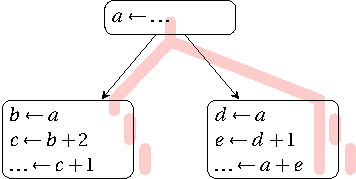
\includegraphics[width=0.55\textwidth]{domtree.pdf}
\caption{\label{fig:alternative_ssa_destruction:fig:domtree}Variables live ranges are sub-trees of the dominator tree\index{dominator!tree}\index{live range, as a dominator sub-tree}}
\end{figure}


\paragraph{Virtualizing $\phi$-related copies}
The last step toward a memory-friendly and fast SSA-destruction algorithm consists in emulating the initial introduction of copies\index{virtual isolation, of \phinode}  and only actually insert them on the fly when they appear to be required. 
We use \emph{exactly the same algorithms as for the solution without virtualization}, and use a special location in the code, identified as a ``virtual'' parallel copy, where the real copies, if any, will be placed.

Because of this we consider a different semantic for \phifuns than the multiplexing mode previously defined. 
To this end we differentiate $\phi$-operands for which a copy cannot be inserted (such as for the \texttt{br\_dec} of Figure~\ref{fig:alternative_ssa_destruction:ex_jump_impossible_b}) to the others. 
We use the term non-split and split operands introduced in Section~\ref{par:alternative_ssa_destruction:strong}. 
For a \phifun $B_0:a_0=\phi(B_1:a_1,\dots,B_n:a_n)$ and a split operand $B_i:a_i$, we denote the program point where the corresponding copy would be inserted as the \emph{early point}\index{early point, of a basic block} of $B_0$ ($\early{B_0}$ -- right after the \phifuns of $B_0$) for the \defop, and as the \emph{late point}\index{late point, of a basic block} of $B_i$ ($\late{B_i}$ -- just before the branching instruction) for a \useop.
\begin{definition}[copy mode]\index{copy mode, semantic of \phiop}}
Let a \phifun $B_0:a_0=\phi(B_1:a_1,\dots,B_n:a_n)$ be in \emph{copy mode}, then the liveness\index{liveness!\phifun} for any split operand follows the following semantic: its \defop is considered to be at the early point\index{basic-block early} of $B_0$, in other words, variable $a_0$ is \emph{not} live-in of $B_0$; its \useops are at the late point\index{basic-block late} of the corresponding predecessor basic-blocks, in other words variable $a_i$ for $i>0$ is (unless used further) \emph{not} live-out of basic block $B_i$. The liveness for non-split operands follows the multiplexing mode semantic. 
\end{definition}

When the algorithm decides that a virtual copy $a'_i \gets a_i$ (resp.~$a_0 \gets a'_0$) cannot be coalesced, it is \emph{materialized}\index{materialization, of copies} in the parallel copy and $a'_i$ (resp. 
$a'_0$) becomes explicit in its merged-set. 
The corresponding \phiop is replaced and the use of $a'_i$ (resp.~def of $a'_0$) is now assumed, as in the multiplexing mode, to be on the corresponding control-flow edge. 
This way, only copies that the first approach would finally leave un-coalesced are introduced. 
We choose to postpone the materialization of all copies along a single traversal of the program at the very end of the de-coalescing process. 
Because of the virtualization of $\phi$-related copies, the de-coalescing scheme given by Algorithm~\ref{alg:alternative_ssa_destruction:domup} have to be adapted to emulate live ranges of split operands. 
The pseudo-code for processing a local virtual variable is given by Algorithm~\ref{alg:alternative_ssa_destruction:virtualdecoalesce}. 
The trick is to use the \phifun itself as a placeholder for its set of local virtual variables. 
As the live range of a local virtual variable is very small, the cases to consider are quite limited: 
a local virtual variable can interfere with another virtual variable (lines~\ref{line:interfvirtual_start}-\ref{line:interfvirtual_end}) or with a ``real'' variable (lines~\ref{line:interfreal_start}-\ref{line:interfreal_end}).

\begin{algorithm}[h]
  \lForEach{$c\in \colors$}{$c.\curidom=\valundef$}
  \ForEach{basic block $B$ in CFG in DFS pre-order of the dominance tree}{
    \ForEach{program point $l$ of $B$ in topological order}{
      \If{$l=\late{B}$}{
        \lForEach{$c\in \colors$}{$c.\curphi=\valundef$}
        \ForEach{basic-block $B'$ successor of $B$}{
          \ForEach{operation Phi: ``$B':a_0=\phi(\dots, B:v,\dots)$'' in $B'$}{
            \lIf{$\neg\colored(\textit{Phi})$}{continue}
            \lElse{$c\gets \col(Phi)$}\;
            \textsf{DeCoalesce\_virtual}(\textit{Phi}, $B:v$, c.\curphi, c.\curidom)\;
            \lIf{$\colored(\textit{Phi})$}{$c.\curphi\gets \textit{Phi}$}\;
          }
        }
      }
      \Else {
        \ForEach{operation \textit{OP} at $l$ (including \phifuns)}{
          \ForEach{variable $v$ defined by \textit{OP}}{
            \lIf{$\neg\colored(v)$}{continue}
            \lElse{$c\gets \col(v)$}\;
            \textsf{DeCoalesce}($v, c.\curidom$)\;
            \lIf{$\colored(v)$}{$c.\curidom \gets v$}\;
          }
        }
      }
    }
  }
  \caption{De-coalescing with virtualization of $\phi$-related copies}
  \label{alg:alternative_ssa_destruction:decoal}
\end{algorithm}



\begin{algorithm}[h]
\Func{DeCoalesce\_virtual(\textit{Phi}, $B:v$, \textit{Phi'}, $u$)}{
  %% \Comment{Finds and set the previous virtual variable of color $c$}
  \If(\Comment*[f]{Interference}){$Phi'\neq\valundef \wedge V(\textsf{operand\_from\_B}(\textit{Phi}'))\neq V(a')$}{ \label{line:interfvirtual_start}
    uncolor $\atomic{\textit{Phi}}$\;
    return\;
  } \label{line:interfvirtual_end}

        %% \Comment{Finds and set the immediate dominator of the local virtual variable}
  \While{$(u \neq \valundef) \bigwedge \left(\neg(u \dominates\ B) \vee \neg\colored(u)\right)$}{\label{line:interfreal_start}
    $u \gets \cidom{u}$\;
  }
  $\cidom{v}\gets u$; 

        
        %% \Comment{Walk up variables that have the same value than $u$} 
  $\eanc{v}\gets \valundef$; $\curanc \gets u$\;
  \While{$\curanc\neq\valundef$}{
    %% \Comment{Find the first one that intersects $v$ with the same color than $u$}
    \While{$\curanc\neq \valundef \bigwedge 
      \neg\left(\colored(\curanc) \wedge \curanc.\textsf{islive}(\textsf{out}(B))\right)$}{
      $\curanc \gets \eanc{\curanc}$\;
    }
    \If(\Comment*[f]{interference}){$\curanc \neq \valundef$}{ 
      \If{preferable to uncolor \textit{Phi}}{
        uncolor $\atomic{\textit{Phi}}$\;
        break\;
      } 
      \Else {
        uncolor $\atomic{\curanc}$\;
        $\curanc \gets \eanc{\curanc}$\;\label{line:interfreal_end}
      }
    }
  }
}
\caption{\label{alg:alternative_ssa_destruction:virtualdecoalesce}Process (de-coalescing) a virtual variable}
\end{algorithm}

        
The overall scheme works as follows: 
(1)~every copy related (even virtual) variables are first coalesced (unless pinning to physical resources forbid it); 
(2)~then merged-sets (identified by their associated color) are traversed and interfering variables are de-coalesced; 
(3)~finally, materialization of remaining virtual copies is performed through a single traversal of all \phifuns of the program: 
whenever one of the two operands of a virtual copy is uncolored, or whenever the colors are different, a copy is inserted.

A key implementation aspect is related to the handling of pinning. 
In particular, for correctness purpose, coalescing is performed in two separated steps. 
First pin-$\phi$-webs have to be coalesced. 
Detection and fix of strong interferences is handled at this point. 
The so obtained merged sets (that contain local virtual variables) have to be identified as atomic i.e., they cannot be separated. 
After the second step of coalescing, atomic merged sets will compose larger merged sets. 
A variable cannot be de-coalesced from a set without de-coalescing its atomic merged-set from the set also. 
Non-singletons atomic merged-sets have to be represented somehow. 
For \phifuns, the trick is again to use the \phifun itself as a placeholder for its set of local virtual variables: 
the pinning of the virtual variables is represented through the pinning of the corresponding \phifun. 
As a consequence, any \phifun will be pinned to all its non-split operands.

Without any virtualization, the process of transforming operand pinning into live range pinning also introduces copies and new local variables pinned together. 
This systematic copy insertion can also be avoided and managed lazily just as for $\phi$-nodes isolation. 
We do not address this aspect of the virtualization here: 
to simplify we consider any operand pinning to be either ignored (handled by register allocation) or expressed as live range pinning.





\paragraph{Sequentialization of parallel copies}          
During the whole algorithm, we treat the copies placed at a given program point as \emph{parallel copies}\index{parallel copy, sequentialization of} , which are indeed the semantics of \phifuns. 
This gives several benefits: 
a simpler implementation, in particular for defining and updating liveness sets, a more symmetric implementation, and fewer constraints for the coalescer. 
However, at the end of the process, we need to go back to standard code, i.e., write the final copies in some sequential order.

As explained in Section~\ref{sec:classical_construction_algorithm:destruction} (Algorithm~\ref{alg:ssadestruction:sequentialization}) the sequentialization of a parallel copy can be done using a simple traversal of a windmill farm shaped graph from the tip of the blades to the wheels. 
Algorithm~\ref{alg:alternative_ssa_destruction_algorithm:para_copies_ser} emulates a traversal of this graph (without building it), allowing to overwrite a variable as soon as it is saved in some other variable.

When a variable $a$ is copied in a variable $b$, the algorithm remembers $b$ as the last location where the initial value of $a$ is available. 
This information is stored into \texttt{loc}($a$). 
The initial value that must be copied into $b$ is stored in \texttt{pred}($b$). 
The initialization consists in identifying the variables whose values are not needed (tree leaves), which are stored in the list \texttt{ready}. 
The list \texttt{to\_do} contains the destination of all copies to be treated. 
Copies are first treated by considering leaves (while loop on the list \texttt{ready}). 
Then, the \texttt{to\_do} list is considered, ignoring copies that have already been treated, possibly breaking a circuit with no duplication, thanks to an extra copy into the fresh variable $n$.

\begin{algorithm}[h]
%\Input{A parallel copy $P$}
%\Blankline
%value $\leftarrow$ \texttt{new} hash table \;
%targets $\leftarrow$ \texttt{new} hash table \;
  \KwData{Set $P$ of parallel copies of the form $a \mapsto b$, $a \neq b$, one extra fresh variable $n$}
\KwOut{List of copies in sequential order}
ready $\leftarrow []$ ;
to\_do $\leftarrow []$ ; pred($n$) $\leftarrow \bot$ \;
\ForAll{$(a \mapsto b) \in P$}{
	loc($b$)$ \leftarrow \bot$ ; pred($a$) $\leftarrow \bot$ \Comment*{initialization}
}

\ForAll{$(a \mapsto b) \in P$}{
	loc($a$) $\leftarrow a$ \Comment*{needed and not copied yet}
	pred($b$) $\leftarrow a$ \Comment*{(unique) predecessor}
        to\_do.push($b$) \Comment*{copy into $b$ to be done}
}

\ForAll{$(a \mapsto b) \in P$}{
	\lIf{loc($b$) = $\bot$}{ready.push($b$) \Comment*{$b$ is not used and can be overwritten}
	}
}
\While{to\_do $\neq []$}{
	\While{ready $\ne []$}{
		$b \leftarrow$ ready.pop() \Comment*{pick a free location}
		$a \leftarrow$ pred($b$) ; $c \leftarrow$ loc($a$) \Comment*{available in $c$}
		\texttt{emit\_copy}($c \mapsto b$) \Comment*{generate the copy}
		loc($a$) $\leftarrow b$ \Comment*{now,
                  available in $b$}
                \lIf{$a=c$ and pred($a$) $\neq \bot$}{
                   ready.push(a) \Comment*{just copied, can be overwritten}}
%		\texttt{del}\ targets[$a$] \;
%		\If{$b \in$ targets.keys()}{
%			available.append($b$) \;
%		}
	}
%	\If{targets.keys() $\neq []$}{
        
        
        $b \leftarrow$ to\_do.pop() \Comment*{look for remaining copy}
        \If{$b =$ loc(pred($b$))}{
%
%

%        $a' \leftarrow$ \texttt{new\_ressource}() \;
          \texttt{emit\_copy}($b \mapsto n$) \Comment*{break circuit with copy}
		loc($b$) $\leftarrow n$ \Comment*{now, available in $n$}
                ready.push($b$) \Comment*{$b$ can be overwritten}
%         \If{$b \in$ targets.keys()}{
%           available.append($b$) \;
%         }
%         values[$b$] $\leftarrow a'$ \;
}
	
}
        \caption{Parallel copy sequentialization algorithm}
        \label{alg:alternative_ssa_destruction_algorithm:para_copies_ser}
\end{algorithm}
%% +Pour l'implémenter on différentie resources et valeurs . La copie a->b%% +signifie que la valeur dans la resource a doit être copiee dans la
%% +resource b.  On racourcit en disant que la valeur ``a'' initialement
%% +dans la resource ``a'' doit être copiee dans la resource
%% +``b''.\\ Ainsi on maintient pour chaque valeur (v) dans quelle
%% +resource elle est disponible (Rcur(v)) et pour chaque resource (r)
%% +quelle valeur (s'il y en a une) elle devra contenir à la fin (Vend(r))
%% +(predecesseur dans le graphe).\\ On construit initialement et
%% +maintient la liste des feuilles ``leaves'' ie de resources qui ne
%% +contiennent pas de valeur (où bien la valeur est disponible
%% +ailleur). On est pour cela obligé de parcourir la liste des valeurs et
%% +marquer les resource qui contiennent une valeur. \\ On construit une
%% +autre liste ``todo'' qui est la liste des resources qui doivent avoir
%% +une valeur à la fin et qui ne contiennent pas cette valeur.\\ Si
%% +leaves n'est pas vide on pull une feuille b, et donc une copie de a->b
%% +avec a=Rcur(Vend(b)). On génère cette copie, et on set
%% +Rcur(Vend(b)):=b (la valeur Vend(b) qui était dans a est maintenant
%% +dans b). a est donc libérée de la valeur Vend et on push  a dans
%% +leaves.\\ Si leaves est vide, c'est soit que c'est terminé, soit qu'il
%% +y a un cycle sans duplication. Dans ce cas, on pull une resource a. Si
%% +Rcur(Vend(a))==a, a a déjà été traité, on passe. Sinon, on est en
%% +présence d'un cycl avec Rcur(a)=a. on génère une nouvelle variable
%% +(resource) a', on genère la copie a->a'. On met à jour Rcur(a):=a'. A
%% +est libéré, on le met dans leaves.

\section{Further Readings}
SSA destruction was first addressed by Cytron et al.~\cite{CFR+91} who propose to simply replace each \phifun by copies in the predecessor basic block. 
Although this naive translation seems, at first sight, correct, Briggs et al.~\cite{BriggsSSA} pointed subtle errors due to parallel copies and/or critical edges in the control-flow graph. 
Two typical situations are identified, namely the ``lost copy problem'' and the ``swap problem''. 
The first solution, both simple and correct, was proposed by Sreedhar et al.~\cite{VC+99}. 
They address the associated problem of coalescing and describe three solutions. 
The first one, consists in three steps: 
(a)~translate SSA into CSSA, by isolating \phifuns; 
(b)~eliminate redundant copies; 
(c)~eliminate \phifuns and leave CSSA. 
The third solution that turns out to be nothing else than the first solution that would virtualizes the isolation of \phifuns shows to introduce fewer copies. 
The reason for that, identified by Boissinot et al., is due to the fact that in the presence of many copies the code contains many intersecting variables that do not actually interfere. 
Boissinot et al.~\cite{Boissinot09} revisited Sreedhar et al.'s approach in the light of this remark and proposed the value based interference described in this chapter.

The ultimate notion of interference was discussed by Chaitin et al.~\cite{Chaitin81} in the context of register allocation. 
They proposed a simple conservative test: 
\emph{two variables interfere if one is live at a definition point of the other and this definition is not a copy between the two variables}. 
This interference notion is the most commonly used, see for example how the interference graph is computed in~\cite{appel:2002:modern}. 
Still they noticed that, with this conservative interference definition, after coalescing some variables the interference graph has to be updated or rebuilt. 
A counting mechanism to update the interference graph was proposed, but it was considered to be too space consuming. 
Recomputing it from time to time was preferred~\cite{Chaitin81,Chaitin82}.

The value-based technique described here can also obviously be used in the context of register allocation even if the code is not under SSA form. 
The notion of value may be approximated using data-flow analysis on specific lattices~\cite{AlpernWZ88} and under SSA form simple global value numbering~\cite{Rosen88} can be used.

Leung and George~\cite{leung:1999:ssa_mach} addressed SSA destruction for machine code. 
Register renaming constraints, such as calling conventions or dedicated registers, are treated with pinned variables. 
Simple data-flow analysis scheme is used to place repairing copies. 
By revisiting this approach to address the coalescing of copies Rastello et al.~\cite{Rastello:2004:CGO} pointed out and fixed a few errors present in the original algorithm. 
While being very efficient in minimizing the introduced copies, this algorithm is quite complicated to implement and not suited for just in time compilation.

The first technique to address speed and memory footprint was proposed by Budimli\'{c} et al.~\cite{Budimlic02}. 
It proposes the de-coalescing technique, revisited in this chapter, that exploits the underlying tree structure of dominance relation between variables of the same merged-set.

Last, this chapter describes a fast sequentialization algorithm that requires the minimum number of copies. 
A similar algorithm has already been proposed by C.~May~\cite{May89}.





